\documentclass[conference]{IEEEtran}
\IEEEoverridecommandlockouts

\usepackage{color}
\usepackage{url}
\usepackage{graphicx}
\usepackage{subfigure}
\usepackage{booktabs}
\usepackage{multirow}
\usepackage{balance}
\usepackage{pifont}
\usepackage[colorlinks,linkcolor=black,urlcolor=black]{hyperref}
\usepackage{amsmath,amssymb,amsfonts}

\graphicspath{{figures/}}
\newcommand{\figref}[1]{Fig.~\ref{#1}}
\newcommand{\tabref}[1]{Table~\ref{#1}}
\newcommand{\secref}[1]{Section~\ref{#1}}

\newcommand{\dong}[1]{\textcolor{blue}{[dong: #1]}}
\newcommand{\libin}[1]{\textcolor{red}{[libin: #1]}}
\newcommand{\zhao}[1]{\textcolor{green}{[zhao: #1]}}

\newcommand{\cmark}{\ding{52}}
\newcommand{\xmark}{\ding{56}}

\begin{document}

\title{Service Mesh: A Simple Survey}

\iffalse
\author{\IEEEauthorblockN{1\textsuperscript{st} Given Name Surname}
  \IEEEauthorblockA{\textit{dept. name of organization (of Aff.)} \\
  \textit{name of organization (of Aff.)}\\
  City, Country \\
  email address}
\and
  \IEEEauthorblockN{2\textsuperscript{nd} Given Name Surname}
  \IEEEauthorblockA{\textit{dept. name of organization (of Aff.)} \\
  \textit{name of organization (of Aff.)}\\
  City, Country \\
  email address}
\and
  \IEEEauthorblockN{3\textsuperscript{rd} Given Name Surname}
  \IEEEauthorblockA{\textit{dept. name of organization (of Aff.)} \\
  \textit{name of organization (of Aff.)}\\
  City, Country \\
  email address}
}
\fi

\maketitle

\begin{abstract}
Microservice architecture is widely used by Internet companies nowadays.
It is designed for the complex services.
Developers can easily deploy and manage a single service.
However, it also raise the complexity of the whole system, which makes the communication components between services bloated.
Service mesh is introduced to improve the management of the large amounts of microserivces.
Regardless of the design and implement of the single service, service mesh can work directly on the container of the service with the help of container technology, e.g. Docker.
In addition to manage the network communication, service mesh also have the various abilities, e.g., service registration and service discovery, of the tradditional microservices architecture.
We presant this paper to make a simple survey on service mesh, to introduce its history and applications.
Besides, we concretely introduce a popular architecture, Istio, to help better understand the principle of service mesh.
\cite{li2019service}
\end{abstract}

\begin{IEEEkeywords}
  Microservices, Service Mesh, Service Oriented Architecture, Istio
\end{IEEEkeywords}

\section{Introduction} \label{sec:intro}
\cite{li2019service}

\section{Service Mesh} \label{sec:mesh}

\section{Istio} \label{sec:istio}
Cloud platforms provide a wealth of benefits for the organizations that use them. However, there’s no denying that adopting the cloud can put strains on DevOps teams. Developers must use microservices to architect for portability, meanwhile operators are managing extremely large hybrid and multi-cloud deployments.\cite{Concepts}
The term service mesh is used to describe the network of microservices that make up such applications and the interactions between them. As a service mesh grows in size and complexity, it can become harder to understand and manage. Its requirements can include discovery, load balancing, failure recovery, metrics, and monitoring. A service mesh also often has more complex operational requirements, like A/B testing, canary rollouts, rate limiting, access control, and end-to-end authentication.
When organizations move to microservices, they need to support dozens or hundreds of specific applications. Managing those endpoints separately means supporting a large number of virtual machines or VMs, including demand. Cluster software like Kubernetes can create pods and scale them up, but Kubernetes does not provide routing, traffic rules, or strong monitoring or debugging tools.
As the number of services increases, the number of potential ways to communicate increases exponentially. Two services have only two communication paths. Three services have six, while 10 services have 90. A service mesh provides a single way to configure those communications paths by creating a policy for the communication.
A service mesh instruments the services and directs communications traffic according to a predefined configuration. That means that instead of configuring a running container (or writing code to do so), an administrator can provide configuration to the service mesh and have it complete that work. This previously always had to happen with web servers and service-to-service communication.\cite{IBM}
Istio is a configurable, open source service-mesh layer that connects, monitors, and secures the containers in a Kubernetes cluster. Istio works natively with Kubernetes only, but its open source nature makes it possible for anyone to write extensions enabling Istio to run on any cluster software.\cite{IBM}
At a high level, Istio helps reduce the complexity of these deployments, and eases the strain on development teams. It is a completely open source service mesh that layers transparently onto existing distributed applications. It is also a platform, including APIs that let it integrate into any logging platform, or telemetry or policy system. Istio’s diverse feature set lets users successfully, and efficiently, run a distributed microservice architecture, and provides a uniform way to secure, connect, and monitor microservices.\cite{Concepts}

\subsection{Benefits of Istio}
The major benefits of a service mesh include capabilities for improved debugging, monitoring, routing, security, and leverage. That is, with Istio, it will take less effort to manage a wider group of services.\cite{Concepts}

\subsubsection{Improved debugging}
For example, that a service has multiple dependencies. The pay claim service at an insurance company calls the deductible amt service, which calls the is member covered service, and so on. A complex dependency chain might have 10 or 12 service calls. When one of those 12 is failing, there will be a cascading set of failures that result in some sort of 500 error, 400 error, or possibly no response at all.
To debug that set of calls, you can use something like a stack trace. On the frontend, client-side developers can see what elements are pulled back from web servers, in what order, and examine them. Frontend programmers can get a waterfall diagram to aid in debugging, as shown in fig.1.\cite{Concepts}
\begin{figure}[htbp]
	\centering
	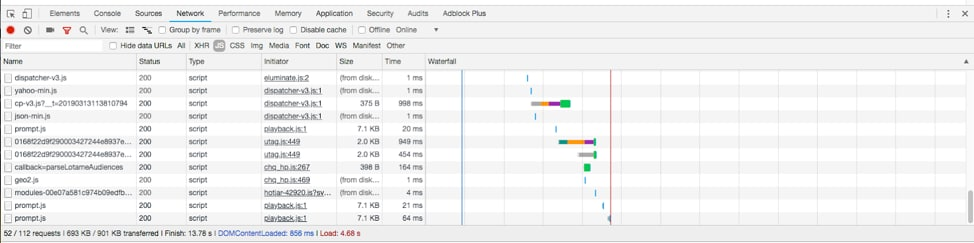
\includegraphics[width=0.5\textwidth]{figure/1.png}
	\caption{Waterfall Diagram\label{fig:1}}
\end{figure}

\subsubsection{Monitoring and observability}
DevOps teams and IT Administration may want to observe the traffic to see latency, time-in-service, errors as a percentage of traffic, and so on. Often, they want to see a dashboard. A dashboard provides a visualization of the sum, or average, or those metrics over time—perhaps with the ability to "drill down" to a specific node, service, or pod. Kubernetes does not provide this functionality natively.\cite{IBM}

\subsubsection{Policy}
By default, Kubernetes allows every pod to send traffic to every other pod. Istio allows administrators to create a policy to restrict which services can work with each other. So, for example, services can only call other services that are true dependencies. Another policy to keep services up is a rate limit, which will stop excess traffic from clogging a service and prevent denial of service attacks.\cite{IBM}

\subsubsection{Routing and load balancing}
By default, Kubernetes provides round-robin load balancing. If there are six pods that provide a microservice, Kubernetes will provide a load balancer, or "service," that sends requests to each pod in increasing order, then it will start over. However, sometimes a company will deploy different versions of the same service in production.

The simplest example of this may be a blue/green deploy. In that case, the software might build an entirely new version of the application in production without sending production users to it. After promoting the new version, the company can keep the old servers around to make switchback quick in the event of failure.

With Istio, this is as simple as using tagging in a configuration file. Administrators can also use labels to indicate what type of service to connect to and build rules based on headers. So, for example, beta users can route to a ‘canary’ pod with the latest and greatest build, while regular users go to the stable production build.\cite{IBM}

\subsubsection{Circuit breaking}
If a service is overloaded or down, additional requests will fail while continuing to overload the system. Because Istio is tracking errors and delays, it can force a pause—allowing a service to recover—after a specific number of requests set by policy. You can enforce this policy across the entire cluster by creating a small text file and directing Istio to use it as a new policy.\cite{IBM}

\subsubsection{Security}
Istio provides identity, policy, and encryption by default, along with authentication, authorization, and audit (AAA). Any pods under management that communicate with others will use encrypted traffic, preventing any observation. The identity service, combined with encryption, ensures that no unauthorized user can fake—or "spoof"—a service call. AAA provides security and operations professionals the tools they need to monitor, with less overhead.\cite{IBM}

\subsubsection{Simplified administration}
Traditional applications still need the identify, policy, and security features that Istio offers. That has programmers and administrators working at the wrong level of abstraction, reimplementing the same security rules over and over for every service. Istio allows them to work at the right level—setting policy for the cluster through a single control panel.\cite{IBM}

\subsection{Architecture}
An Istio service mesh is logically split into a data plane and a control plane.\cite{IBM}
\subsubsection{The data plane}
The data plane is composed of a set of intelligent proxies (Envoy) deployed as sidecars. These proxies mediate and control all network communication between microservices along with Mixer, a general-purpose policy and telemetry hub.\cite{Concepts}
\subsubsection{The control plane}
The control plane manages and configures the proxies to route traffic. Additionally, the control plane configures Mixers to enforce policies and collect telemetry.\cite{Concepts}

fig.2 shows the different components that make up each plane:
\begin{figure}[htbp]
	\centering
	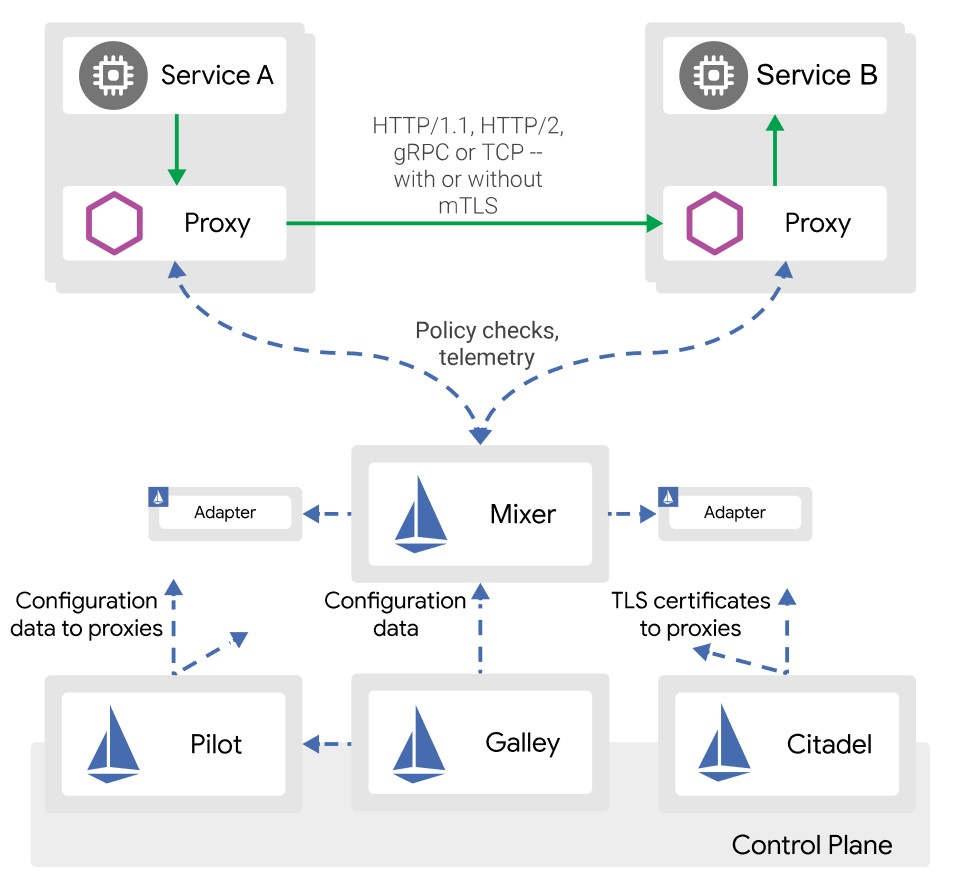
\includegraphics[width=0.5\textwidth]{figure/2.jpg}
	\caption{Istio Architecture\label{fig:2}}
\end{figure}

\subsection{Example}
This example deploys a sample application composed of four separate microservices used to demonstrate various Istio features. The application displays information about a book, similar to a single catalog entry of an online book store. Displayed on the page is a description of the book, book details (ISBN, number of pages, and so on), and a few book reviews.\cite{bookinfo}
The Bookinfo application is broken into four separate microservices:
\subsubsection{productpage}
The productpage microservice calls the details and reviews microservices to populate the page.

\subsubsection{details The details microservice contains book information.}
The details microservice contains book information.

\subsubsection{reviews}
The reviews microservice contains book reviews. It also calls the ratings microservice.

\subsubsection{ratings}
The ratings microservice contains book ranking information that accompanies a book review.\cite{bookinfo}

The end-to-end architecture of the application is shown in fig.3.
\begin{figure}[htbp]
	\centering
	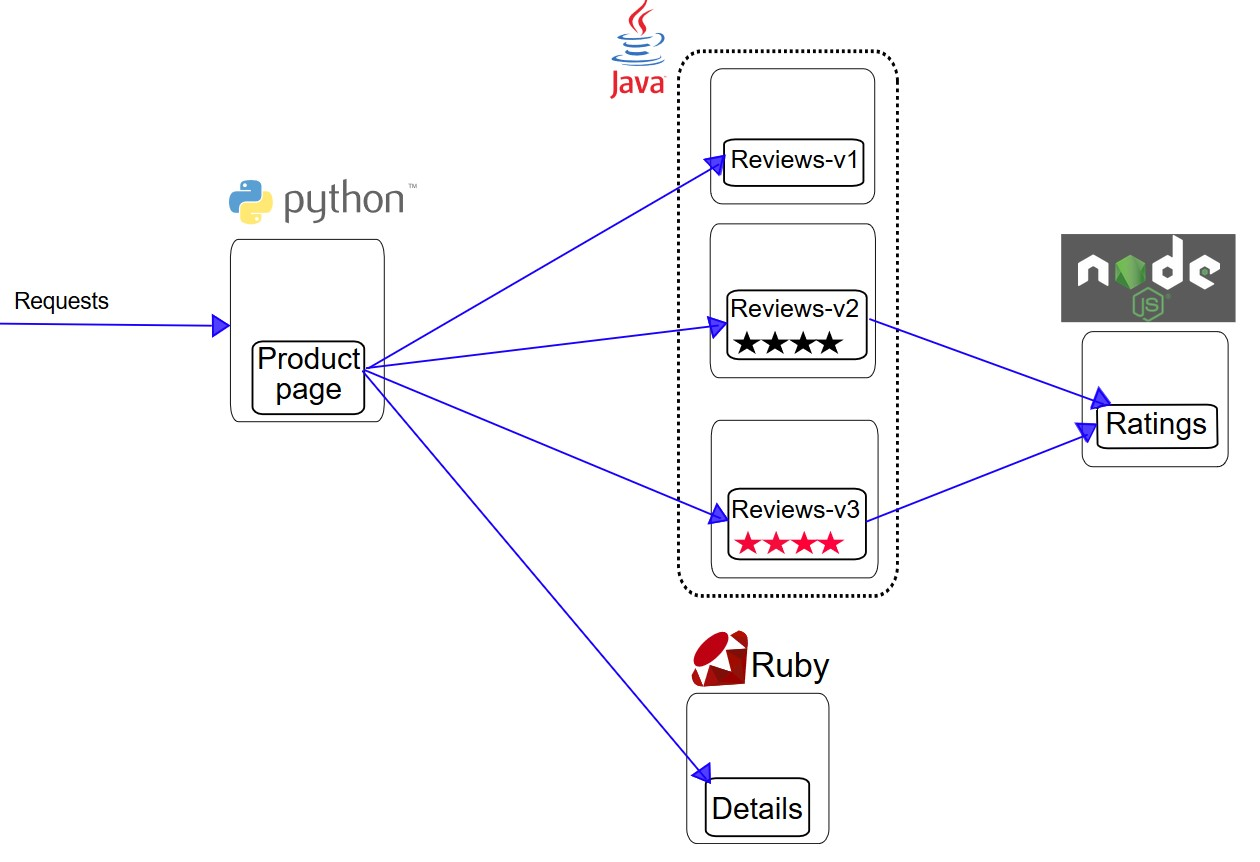
\includegraphics[width=0.5\textwidth]{figure/3.jpg}
	\caption{Bookinfo Application without Istio\cite{bookinfo}\label{fig:3}}
\end{figure}\par

To run the sample with Istio requires no changes to the application itself. Instead, we simply need to configure and run the services in an Istio-enabled environment, with Envoy sidecars injected along side each service. The needed commands and configuration vary depending on the runtime environment although in all cases the resulting deployment will be shown in fig.4.

\begin{figure}[htbp]
	\centering
	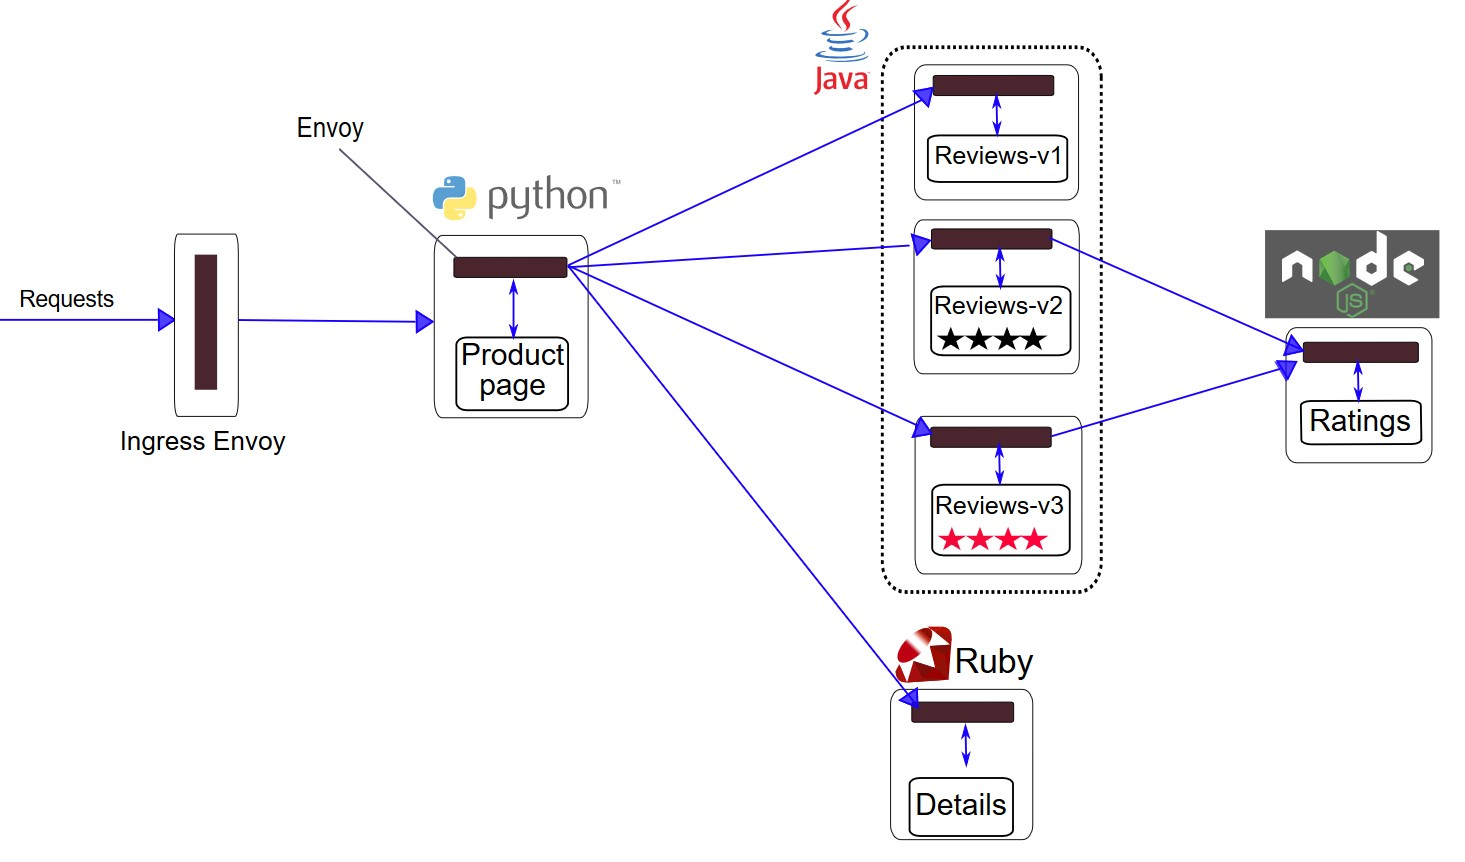
\includegraphics[width=0.5\textwidth]{figure/4.jpg}
	\caption{Bookinfo Application\cite{bookinfo}\label{fig:4}}
\end{figure}

All of the microservices will be packaged with an Envoy sidecar that intercepts incoming and outgoing calls for the services, providing the hooks needed to externally control, via the Istio control plane, routing, telemetry collection, and policy enforcement for the application as a whole.\cite{bookinfo}


\section{Applications} \label{sec:app}

\section{Conclusion}
While service mesh adoption in the cloud native ecosystem is growing rapidly, there is an extensive and exciting roadmap ahead still to be explored. The requirements for serverless computing (e.g. Amazon’s Lambda) fit directly into the service mesh’s model of naming and linking, and form a natural extension of its role in the cloud native ecosystem. The roles of service identity and access policy are still very nascent in cloud native environments, and the service mesh is well poised to play a fundamental part of the story here. Finally, the service mesh, like TCP/IP before it, will continue to be pushed further into the underlying infrastructure. Just as Linkerd evolved from systems like Finagle, the current incarnation of the service mesh as a separate, user-space proxy that must be explicitly added to a cloud native stack will also continue to evolve.

\bibliographystyle{IEEEtran}
\bibliography{mybib}

\end{document}